The global temperature of the earth has been increasing exponentially over the past 100 years \cite{crowley2000causes}. 
Temperatures are expected to keep increasing for at least the next 30 years unless changes are made now to the emissions of greenhouse gas~\cite{UCAR,university_of_alaska_2016}.
Below is a graph illustrating the annual deviation of global surface temperature from the 20$^{\text{th}}$ century average of 13.9$^{\circ}$C.
\begin{figure}[H]
    \centering
    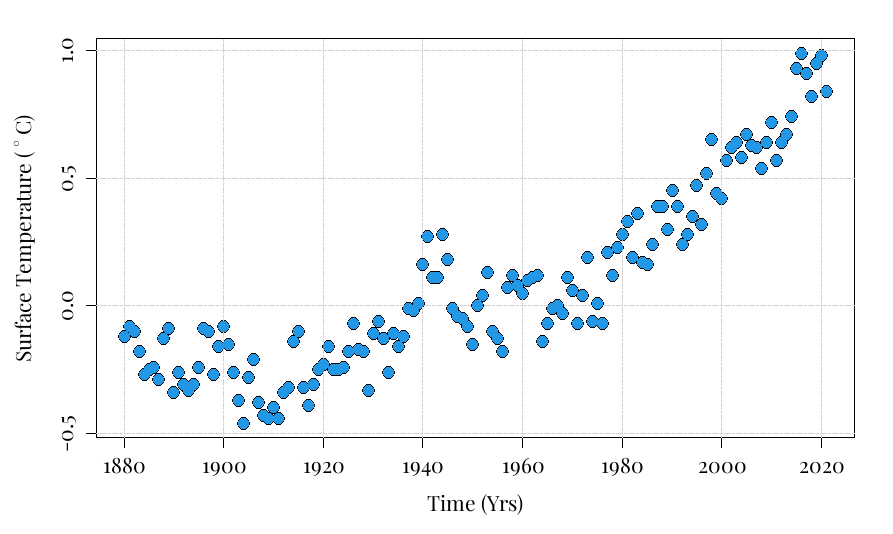
\includegraphics[width=14cm]{LaTeX/Pictures/SST/Global Temp.png}
    \caption{\singlespacing
    Scatter plot of the average annual global temperatures compared to the 20$^{\text{th}}$ century average.}
    \label{fig:noaasurf}
\end{figure}
The data for \figureautorefname~\ref{fig:noaasurf} comes from the National Oceanic and Atmospheric Administration (NOAA)~\cite{NOAA}. 
Any points below 0$^{\circ}$C represent the years when temperatures were less than 13.9$^{\circ}$C, and the points above 0$^{\circ}$C represent the years when temperatures were greater than 13.9$^{\circ}$C.
% Judging from \figureautorefname~\ref{fig:noaasurf}, there seems to be some sense of slowing down after 2010 which aligns with statements made by the EPA, that there has been a recent reduction in the emissions of carbon dioxide \cite{epagreen}.
The earth's surface temperature appears to decrease from 1880 to 1910, then increases exponentially to a little after 1940.
From here, the temperature decreases by approximately $0.05^{\circ}$C entering 1965 before increasing again to the present.
% These dates align closely with the time period of both World Wars, which forced an increase in production.
% We hypothesize that the spike in global surface temperature could be the result of both World Wars.
% The graph above shows that the earth's temperature decreases from 1880 till about 1910 before increasing almost exponentially to the present.
Starting around 1970 to the present, global surface temperatures appear to increase linearly.
While an exponential regression model can be used to fit the data, a quadratic model would seem to work better because of the initial decrease from 1880 to 1910.
The quadratic model would look like
\begin{equation}\label{eq:SSTmodel}
    T(t) = at^2 + bt + c,
\end{equation}
where $a=7.95*10^{-4},\; b=-30.25*10^{-2},\;\text{and } c=287.57$. The response variable, $T(t)$, represents temperature with the units, $^{\circ}$C, that is dependent on time, $t$, expressed in years.
This function seems to fit the data well with the graph below.
\begin{figure}[H]
    \centering
    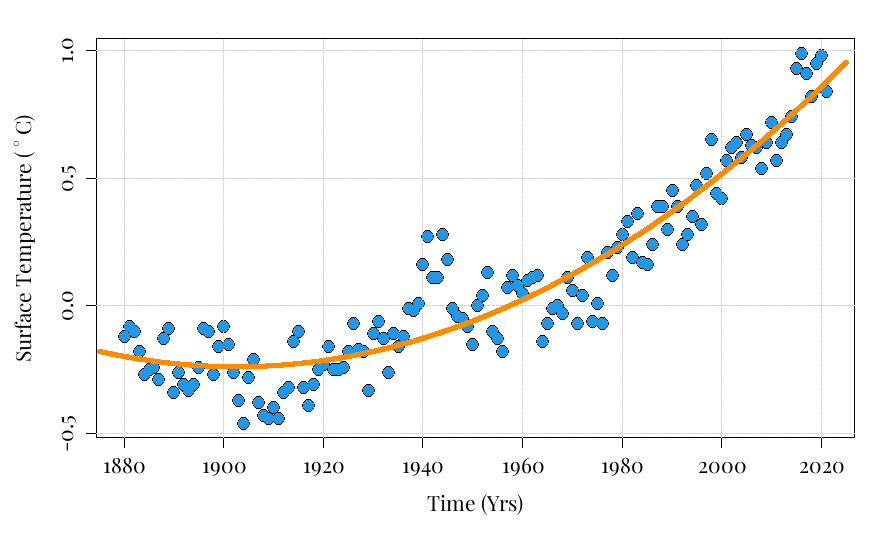
\includegraphics[width=14cm]{Pictures/SST/Global Temp Fit.png}
    \caption{\singlespacing
    Plot of the quadratic function, $T(t)$, on top of the scatter plot given in \figureautorefname~\ref{fig:noaasurf}.}
    \label{fig:polyfitsurf}
\end{figure}
There is a possible issue that should be explored before continuing.
This model projects the change in global  surface temperatures of the earth, but salmon live in the ocean. 
So, designing a model to fit the earth's change in surface temperature over time might not accurately reflect the environmental temperatures of this species.
The National Oceanic and Atmospheric Administration also collect data on the global sea surface temperature over the same time period~\cite{NOAA}.
Below is a graph looking at the global sea surface temperature anomalies with respect to the 20$^{\text{th}}$ century average of 13.9$^{\circ}$C.
\begin{figure}[H]
    \centering
    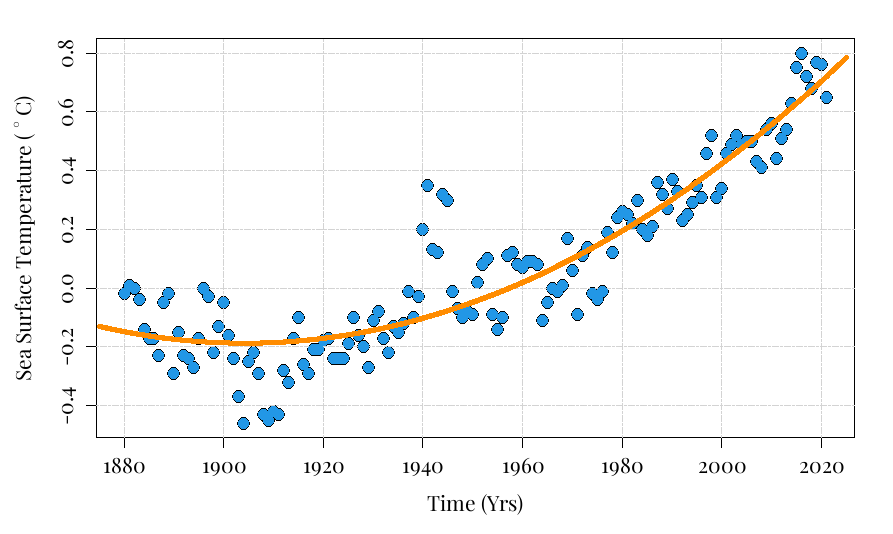
\includegraphics[width=14cm]{Pictures/SST/Global SST Fit.png}
    \caption{\singlespacing
    Scatter plot of the average annual sea surface temperatures compared to the 20$^{\text{th}}$ century average fitted with the quadratic function, $T(t)$, with new coefficients.}
    \label{fig:polyfitSST}
\end{figure}
Since the graph above has a similar trend to \figureautorefname~\ref{fig:noaasurf}, a quadratic model seems to fit this data well.
The new parameters for the quadratic model are, $a=6.67*10^{-5},\; b=-0.25,\; \text{and } c=241.53$.
Looking at \figureautorefname~\ref{fig:polyfitSST} after 1970, the trend appears linear, which means the quadratic equation may not be the best choice for predicting temperature.
Because of this, we will look at sea surface temperatures (SST) after 1970.
Also, Alaska is ranked 40$^{\text{th}}$ in the nation with total greenhouse gas emissions, which may affect that region's SST trend differently than other regions~\cite{adec_2018}.

Alaska has a large number of river streams, but salmon can be seen predominately in the southern parts of Alaska, such as Anchorage, the Kenai Peninsula, near Juneau, and Alaska Peninsula \cite{ADFG}. 
According to the ADFG, salmon swim in these streams from June to September \cite{ADFG}.
Therefore, we sampled water temperature data in these regions during these months to model the change in temperature over time. The data was provided by the United States Geological Survey (USGS)~\cite{usgs_2022}.
When using the USGS database, there are plenty of streams where the Alaskan government was collecting data, but there are a few issues when looking at the data sets for some of the streams~\cite{usgs_2022}.
First, most data sets are a small duration of a few years, which is not enough time to model a trend.
Second, some data sets are missing data for a couple of months every year or even just had big gaps for several years. 
We set criteria for the rivers we wanted to sample; each river needed consistent data for at least 15 years during the months when salmon swim upstream.
In the end, only 5 data sets are usable for analyzing trends over time. 
The 5 streams we use for this analysis are Cooper Creek on the Kenai Peninsula, Kenai River at Cooper Landing, Russell Creek on the Alaska Peninsula, Terror River, just south of the Alaska Peninsula, and Staney Creek which is south of Juneau.
We initially combined the data for each river and calculated the average water temperature per year.
\begin{figure}[H]
    \centering
    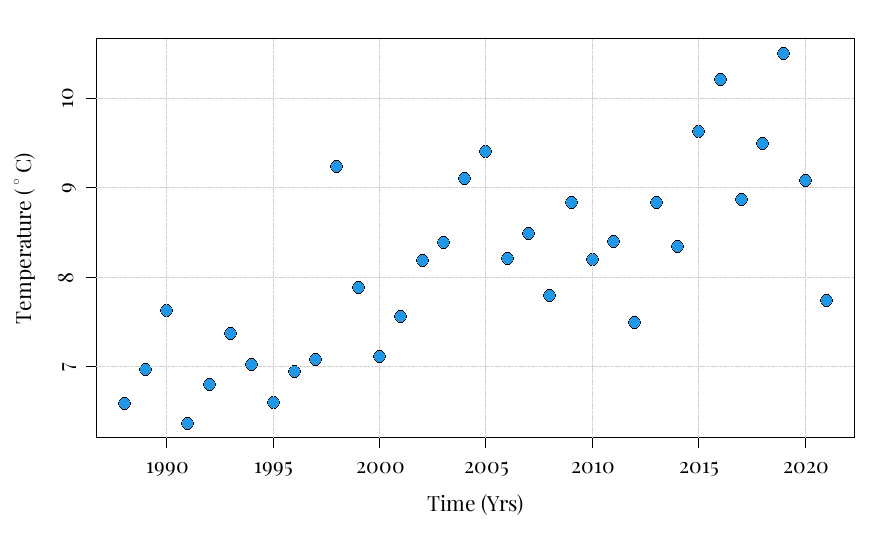
\includegraphics[width=14cm]{Pictures/SST/Alaskan Water Temp.png}
    \caption{\singlespacing
    Scatter plot of the average annual water temperatures during the months of June to September for the combined data of the rivers; Cooper Creek, Kenai River, Russell Creek, Terror River, and Staney Creek. }
    \label{fig:alaskatemp}
\end{figure}
\figureautorefname~\ref{fig:alaskatemp} shows that the trend for the average water temperature per year is fluctuating between increasing and decreasing from 1988 to 2021.
Overall, the data appears to be increasing for the past 33 years.
From \figureautorefname~\ref{fig:alaskatemp}, we can see that, on average, the water temperature is consistently increasing.
This may imply that a linear regression model would fit the data well.
Before fitting the combined river data with a linear model, we have to make sure that each river's change in water temperature over time appears to be increasing linearly.
Below are the plots of each stream fitted with a linear model that closely represents their trend. 
\begin{figure}[H]
    \centering
    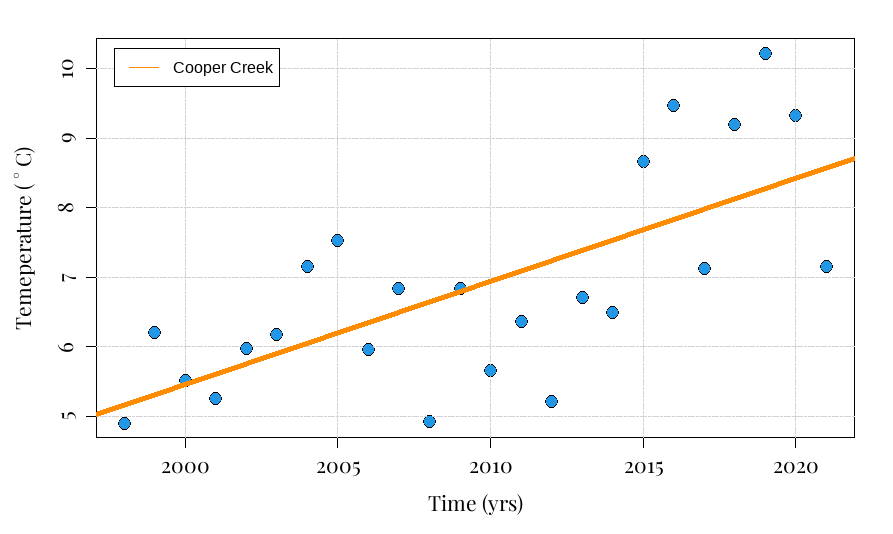
\includegraphics[width=7cm]{Pictures/SST/sst - cooper.png}
    \hfill
    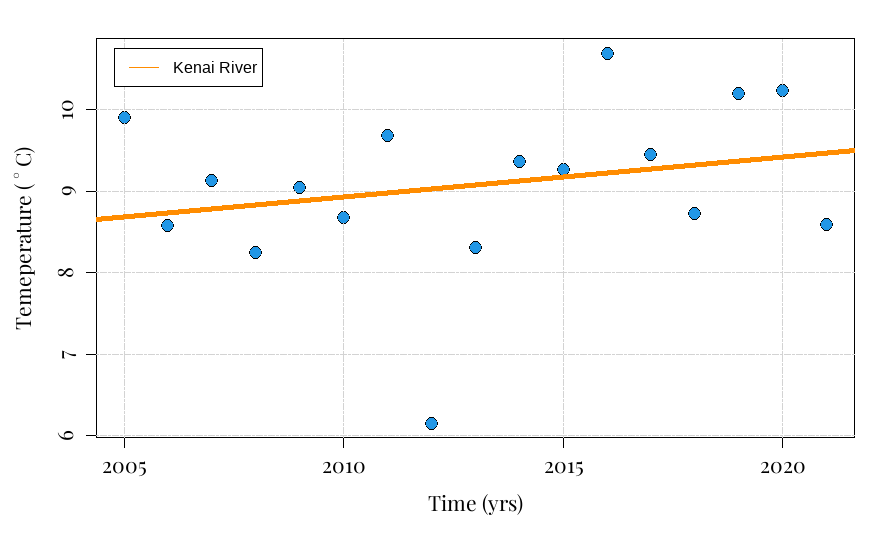
\includegraphics[width=7cm]{Pictures/SST/sst - kenai river.png}
    \\
    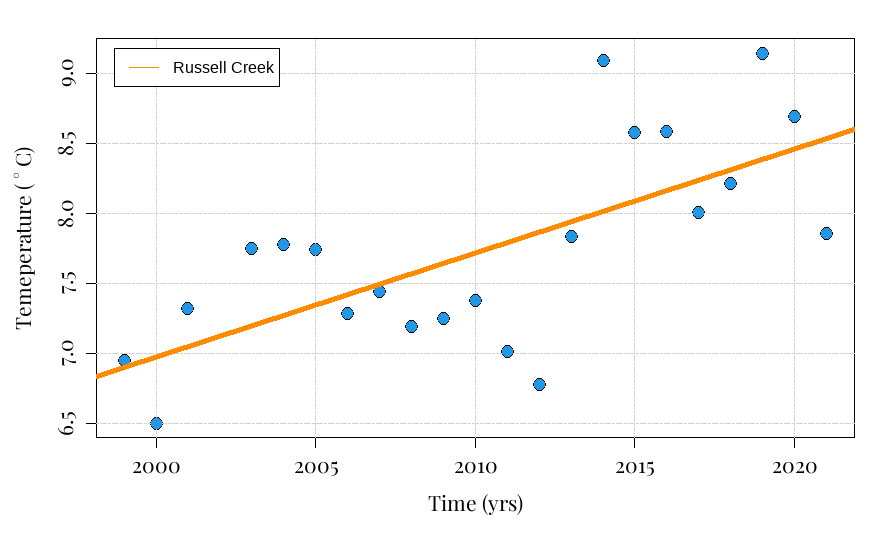
\includegraphics[width=7cm]{Pictures/SST/sst - russell.png}
    \hfill
    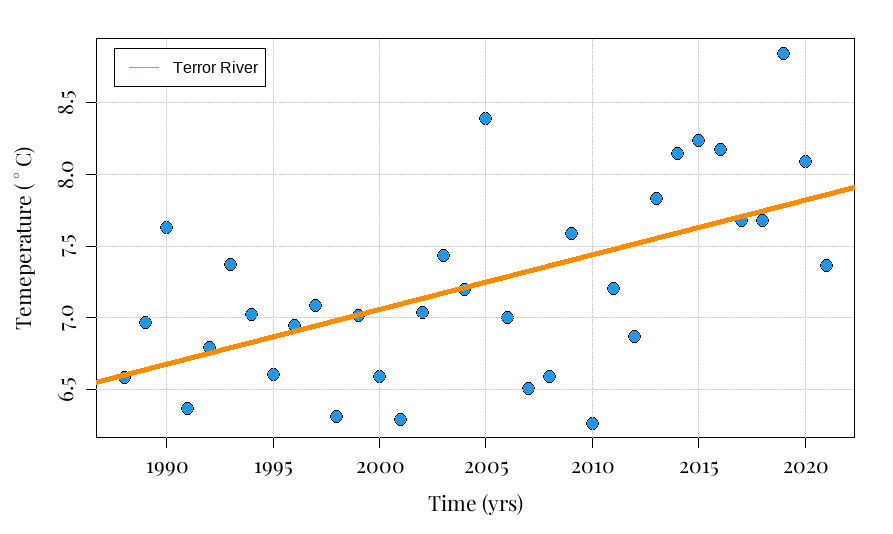
\includegraphics[width=7cm]{Pictures/SST/sst - terror.png}
\end{figure}
\begin{figure}[H]
    \centering
    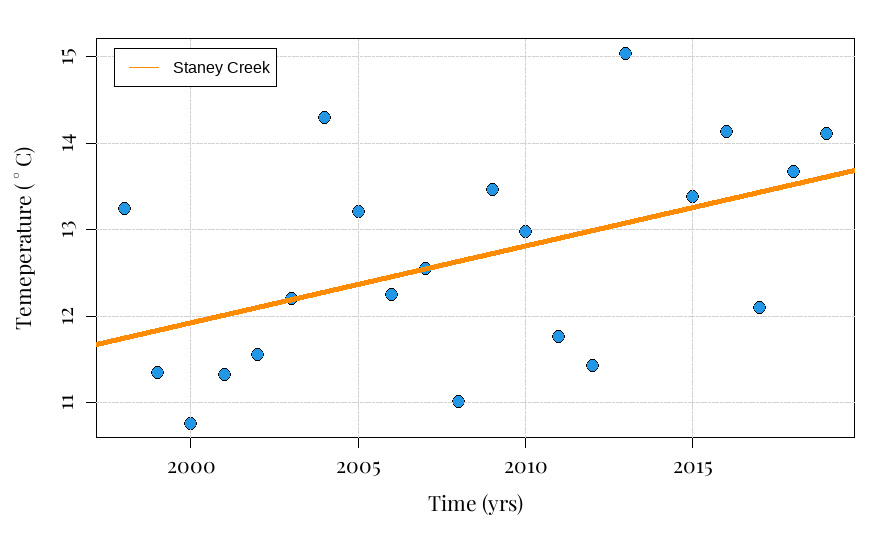
\includegraphics[width=8cm]{Pictures/SST/sst - staney.png}
    \caption{\singlespacing
    Plots of each river's average annual water temperature trend, fitted with a linear model.}\label{fig:sstrivers}
\end{figure}
Notice in \figureautorefname~\ref{fig:sstrivers}, the time span of the recorded water temperatures for some of the rivers are different.
This could cause the combined data used in \figureautorefname~\ref{fig:alaskatemp} to be biased towards rivers with a longer time span.
We can compare the average increase in water temperature for \figureautorefname~\ref{fig:alaskatemp} to the average of the slopes for the rivers in \figureautorefname~\ref{fig:sstrivers}. If the data is biased, we should be able to see it in the comparison.
Each river has a similar trend to the combined data in \figureautorefname~\ref{fig:alaskatemp} with the mean of their slopes representing an average increase in annual water temperature of 0.0797 $^{\circ}$C per year.
When fitting a linear model to \figureautorefname~\ref{fig:alaskatemp} the average increase in water temperature is 0.0803 $^\circ$C per year.
\begin{figure}[H]
    \centering
    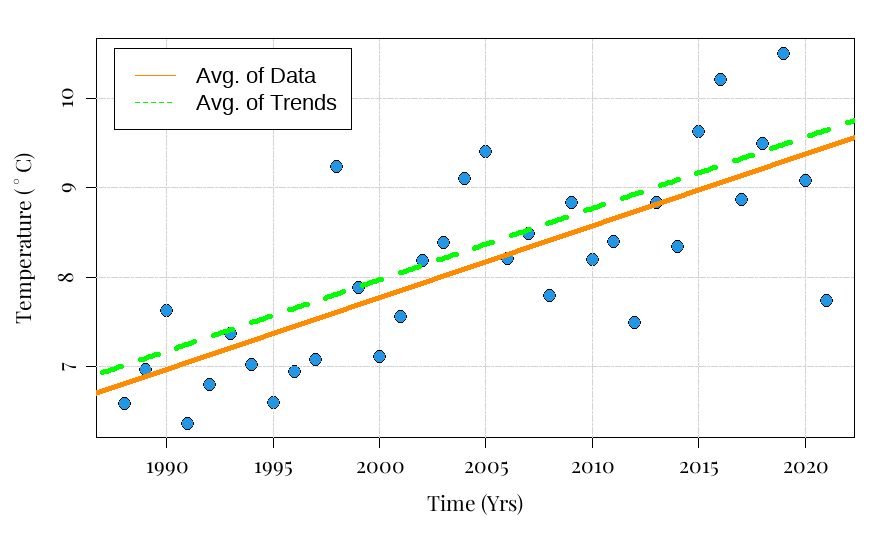
\includegraphics[width=14cm]{LaTeX/Pictures/SST/AlaskaWaterFit.png}
    \caption{\singlespacing
    The solid line represents the average change in annual water temperature of the combined data for the 5 rivers seen in \figureautorefname~\ref{fig:alaskatemp}.
    % the trend of the average water temperature in Alaska for the past 33 years. 
    The dashed line represents the average of the slopes from each river's linear model seen in \figureautorefname~\ref{fig:sstrivers}. 
    % trend for each stream that was sampled in Alaska.
    }
    \label{fig:alaskatempfit}
\end{figure}
The figure above illustrates that for the past 33 years the average change in Alaskan river temperature during the months of salmon spawning migration has a linear growth of approximately 0.08 $^\circ$C per year.
The model for the change in water temperature in Alaska can now be represented as
\begin{equation}\label{eq:sstmodel}
    T(t) = a*t + b,
\end{equation}
with $a=0.08$ and $b = 9.54$. 
The coefficient, $a$, represents the average increase in water temperature over time, and the intercept, $b$, represents 
% the initial water temperature in Alaska about 2000 years ago, and $t$ represents the time in years with an initial starting point 0 B.C. 
% Obviously, the average temperature in Alaskan rivers and creeks 2000 years ago was not $-152.9~^\circ$C, so the linear regression model is only useful for short time periods.
% Thus, letting $b = 9.54$ changes 
the average water temperature for the year 2022.
We will use this model to predict water temperatures in Alaska during the months when salmon migrate to spawning locations.
Now, substituting the function $T(t)$ for the parameter $T$ in \equationautorefname~\eqref{eq:RepoFunLog} gives us
\begin{equation}\label{eq:SalmonRepo}
    \begin{aligned}
        R(T(t)) =\ln\scalebox{1.2}{$\pmb[$}0.32*5*P(T(t))\scalebox{1.2}{$\pmb]$}&= \ln\left(\frac{0.32*5}{1+c(T(t)-T_{opt})^4}\right)\\[.3cm]
        &= \ln\left(\frac{0.32*5}{1+c(at+b-T_{opt})^4}\right).
    \end{aligned}
\end{equation}
Then, substituting in all the parameter values gives the following equation,
\begin{equation}\label{eq:SalmonGrowthTime}
    R(t) = \ln\left(\frac{0.32*5}{1+10^{-4}(0.08t-2.96)^4}\right).
\end{equation}
In \equationautorefname~\eqref{eq:fishexpdif} the growth rate, $r_x$, was revealed after taking the derivative of \equationautorefname~\eqref{eq:fishexp}.
So, by replacing $r_x$ in \equationautorefname~\eqref{eq:fishexp} with $R(t)$ we get
\begin{equation*}
    x(t) = x_0e^{R(t)t}.
\end{equation*}
Then, taking the derivative produces the following,
\begin{equation*}
    \begin{aligned}
        \frac{dx}{dt} &= \pmb[ R(t)+R'(t)t \pmb]x_0e^{R(t)t} = \pmb[ R(t)+R'(t)t \pmb]x,
    \end{aligned}
\end{equation*}
where
\begin{equation}
    R'(t) = \frac{d}{dt}\ln(0.32*5*P(t)) = \frac{P'(t)}{P(t)}.
\end{equation}
As briefly shown in \equationautorefname~\eqref{eq:SalmonRepo}, $P(T)$ from \equationautorefname~\eqref{eq:SurvivalProportionFun} can be rewritten as a function of time using \equationautorefname~\eqref{eq:SSTmodel},
\begin{equation}\label{eq:Repodiff}
    P(t) = \scalebox{1.3}{$\frac{1}{1+10^{-4}(0.08t-2.96)^4}$},\\
\end{equation}
where
\begin{equation}
    P'(t) = \scalebox{1.3}{$\frac{-4*10^{-4}*0.08(0.08t-2.96)^3}{\left(1+10^{-4}(0.08t-2.96)^4\right)^2}$}.\\
\end{equation}
So, the growth rate function can now be written as
\begin{equation}
    G(t) = \ln\left(\frac{0.32*5}{1+10^{-4}(0.08t-2.96)^4}\right) - \scalebox{1.3}{$\frac{4*10^{-4}*0.08t(0.08t-2.96)^3}{1+10^{-4}(0.08t-2.96)^4}$},
\end{equation}
or in a more simplified form,
\begin{equation}\label{eq:GrowthRate}
    G(t) = R(t) + \frac{P'(t)t}{P(t)}.
\end{equation}
To better understand what the growth rate function is doing, we graph the function below.
\begin{figure}[H]
    \centering
    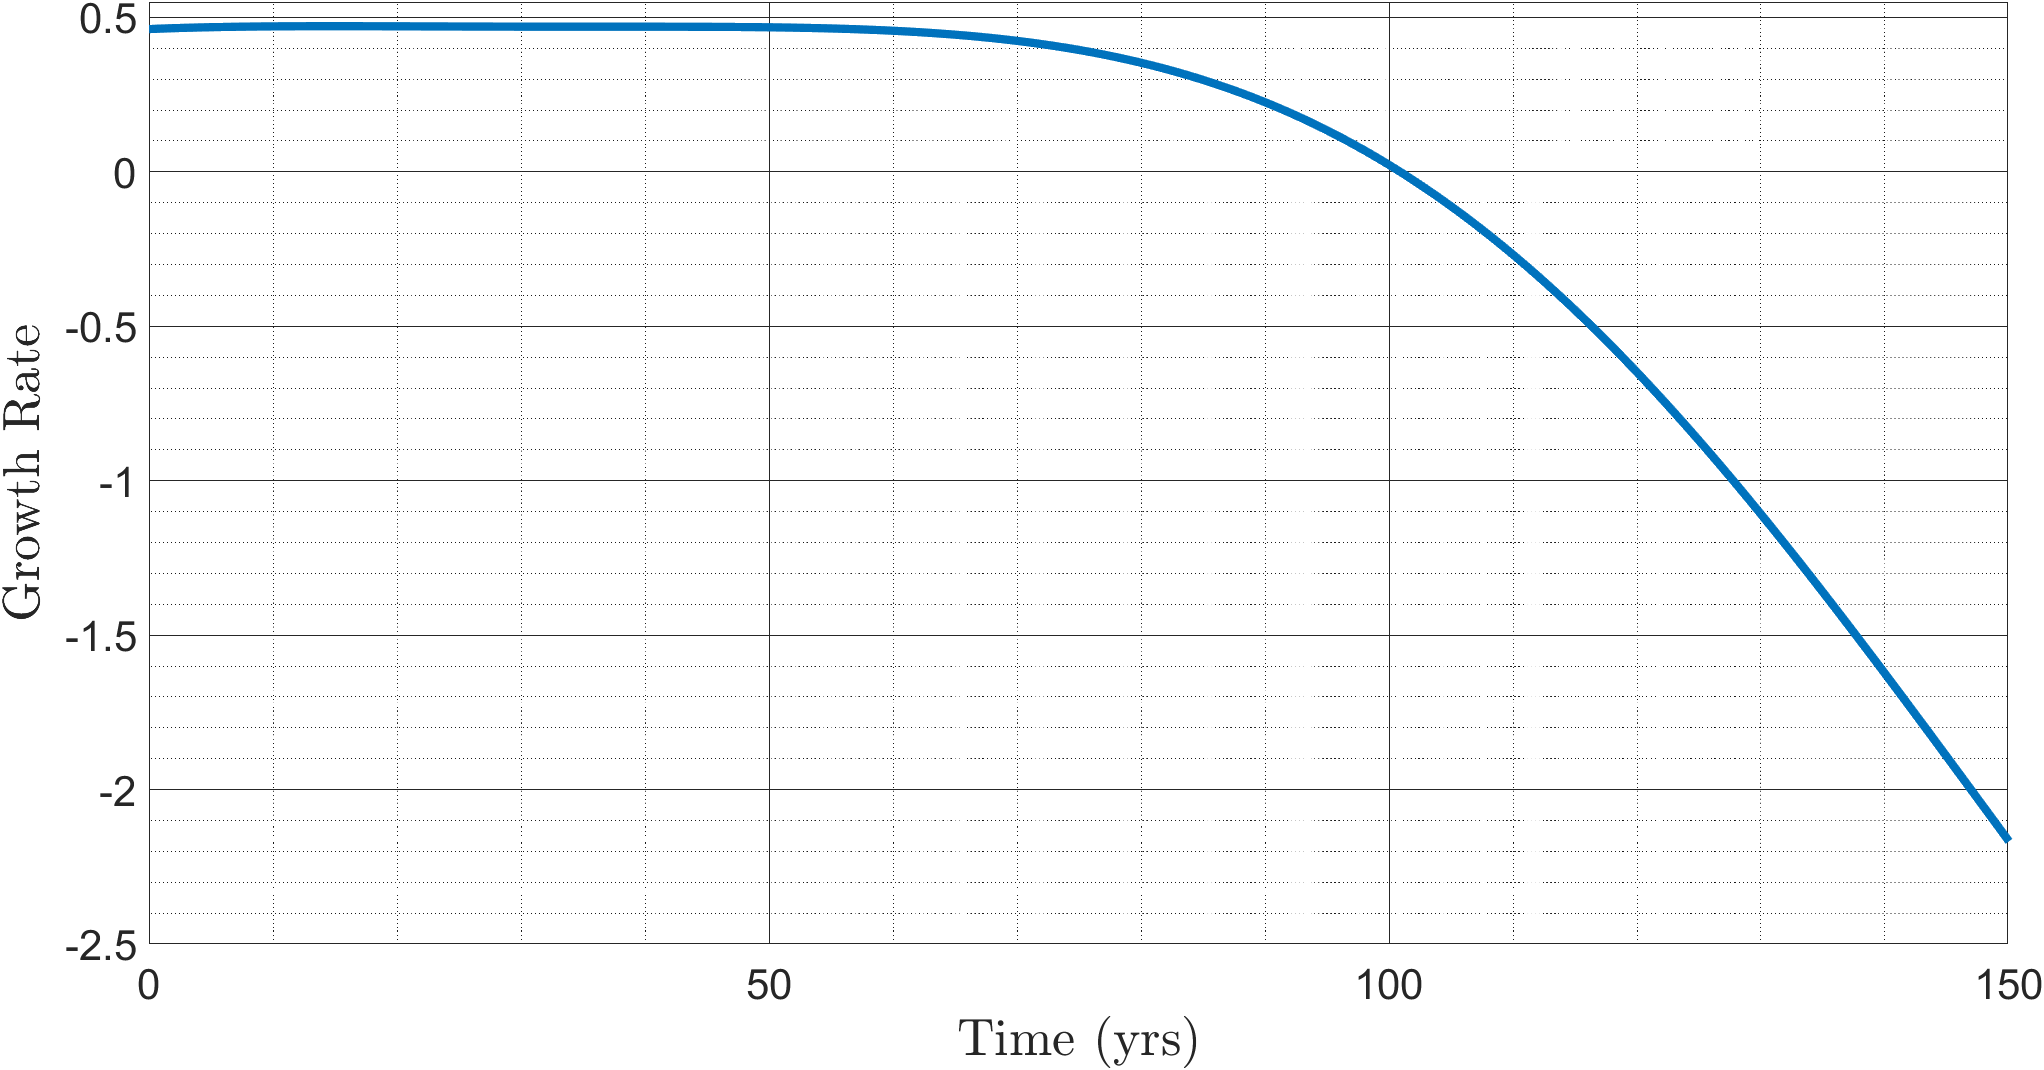
\includegraphics[width=14cm]{Pictures/Salmon Pop/GrowthRateFun.png}
    \caption{\singlespacing
    Plot of the growth rate function, \equationautorefname~\eqref{eq:GrowthRate}, over a time span of 150 years.}
    \label{fig:GrowthRateFunction}
\end{figure}
We can see in the figure above that the growth rate remains positive for approximately the first 100 years. 
After this, the growth rate becomes negative indefinitely.
Now, as shown below, we can substitute the above growth rate function into \equationautorefname~\eqref{eq:salmonlogisticrepo}.
\begin{equation}\label{eq:SalmonLogTime}
    \frac{dx}{dt} = G(t)x\left(1-\frac{x}{K_x}\right).
\end{equation}
Since the model for the salmon population is now dependent on time, it becomes a non-autonomous ordinary differential equation. When comparing this model to \equationautorefname~\eqref{eq:salmonlogisticrepo}, the below figure is produced.
\begin{figure}[H]
    \centering
    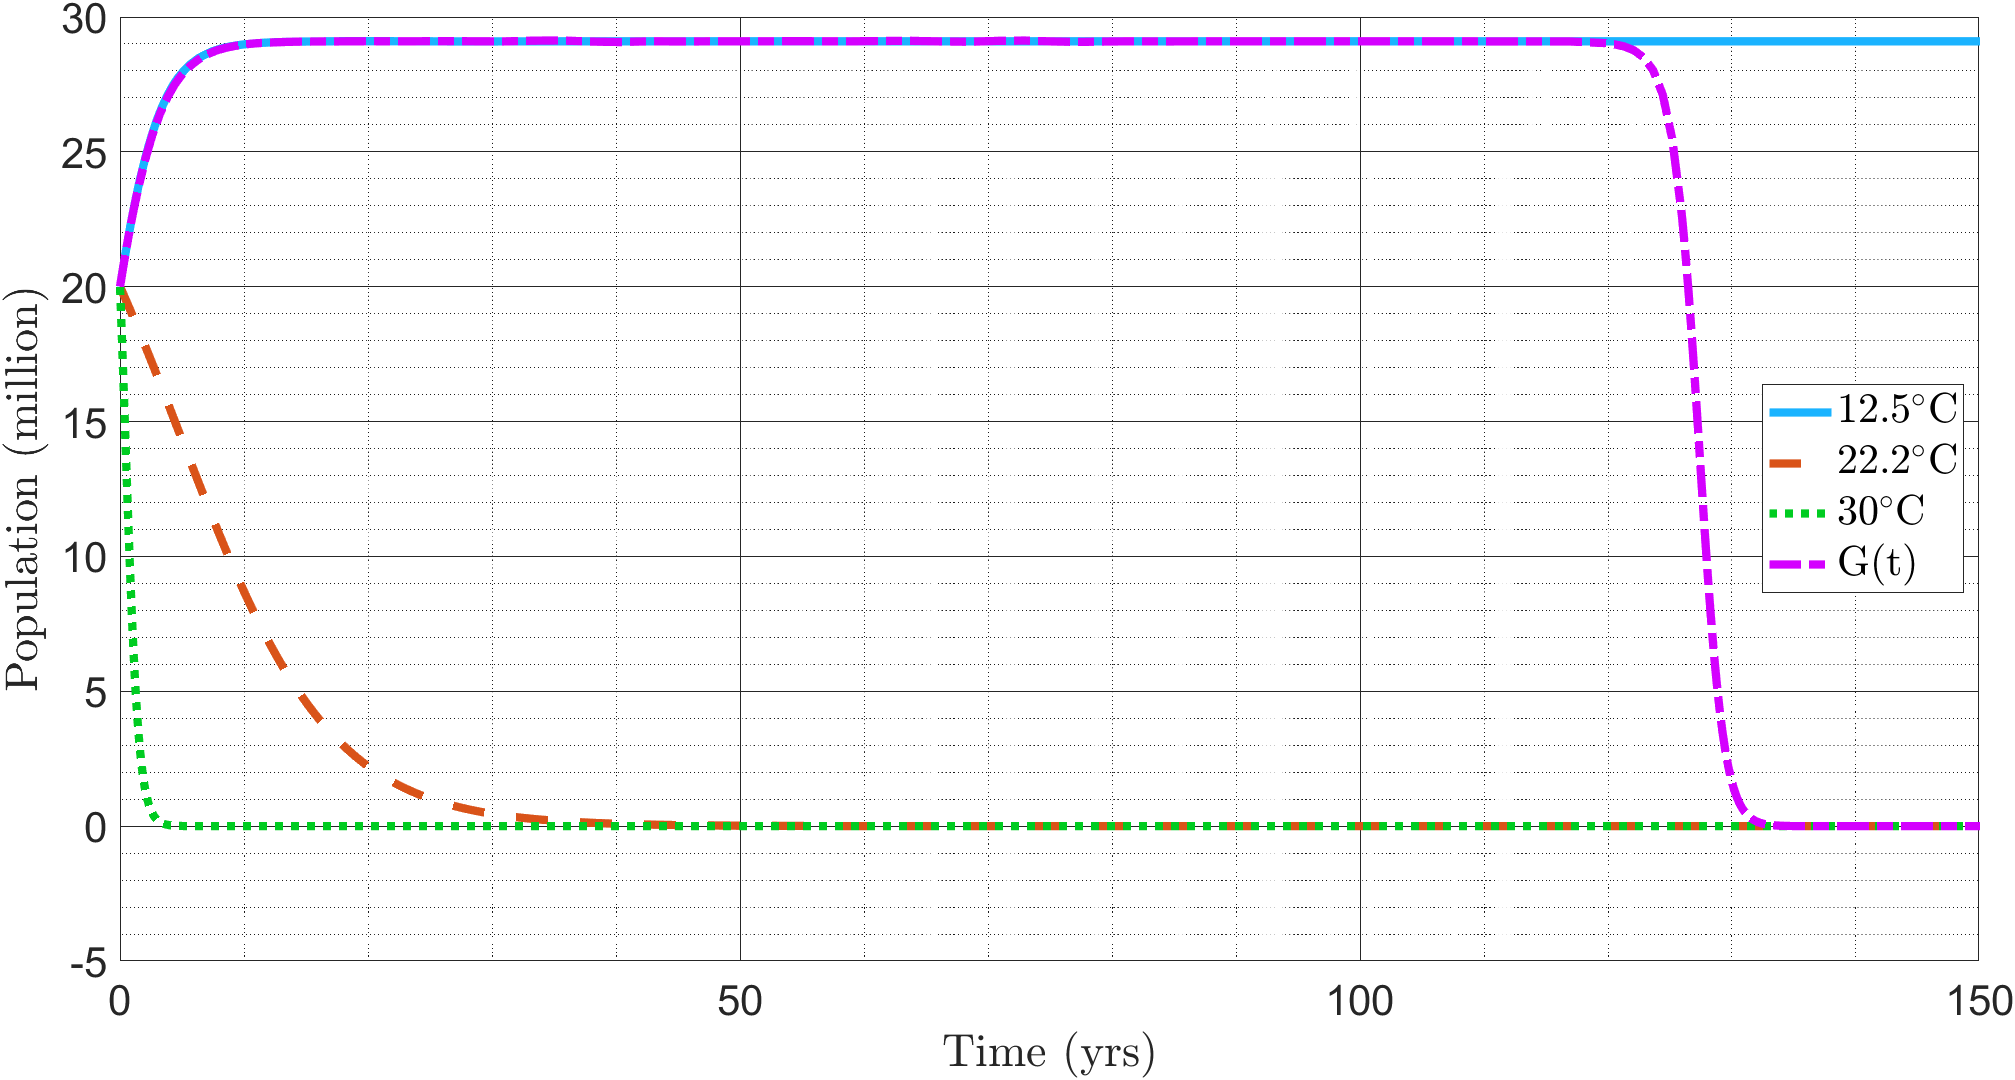
\includegraphics[width=14cm]{Pictures/Salmon Pop/salmon repo model/SalmonWithRepoFun.png}
    \caption{\singlespacing
    Solutions to the autonomous system for some values of water temperature $T$, and the non-autonomous system as a function of time.
    % This figure plots the solutions to \equationautorefname~\eqref{eq:SalmonLogTime}onto \figureautorefname~\ref{fig:salmnologistic}. Also, compared to \figureautorefname~\ref{fig:salmnologistic} the x-axis limits are expanded to illustrate the decline in the salmon population as time gets large.
    }
    \label{fig:SalmonWithRepoFun}
\end{figure}
Using the \textbf{vpasolve} function in MATLAB, we found that in approximately 101 years, the growth rate will change from positive to negative, which is the beginning of the population's descent.
When substituting $t=101$ into \equationautorefname~\eqref{eq:sstmodel}, we get $T(101) = 17.62^{\circ}$C.
This temperature can be denoted as our inflection temperature for the salmon population.
\figureautorefname~\ref{fig:SalmonWithRepoFun} suggests that the water temperature will be too hot for the salmon population in the future, resulting in their death or regional extinction.


